%===============================================================================
%===============================================================================
%
\clearpage
%
\subsection{Example-0302-u \texttt{[COMPILES]}}
%
Example uses user-defined simplex meshes in CHeart mesh format with
quadratic/linear interpolation for velocity/pressure
and solves a dynamic problem.

Setup is the well-known lid-driven cavity problem
on the unit square or unit cube in two and three dimensions.

Current issue: does not converge after 30 some time iterations.
%
%===============================================================================
%
\subsubsection{Mathematical model - 2D}
%
We solve the incompressible Navier-Stokes equation,
%
\begin{align}
    \partial_{t} (\rho \boldsymbol{v}) + \nabla \cdot (\rho \boldsymbol{v} \otimes \boldsymbol{v} + p \boldsymbol{I}) = \rho \boldsymbol{f} & &&\Omega = [0, 1] \times [0, 1], \\
    \nabla \cdot \boldsymbol{v} = 0,
\end{align}
%
with boundary conditions
%
\begin{align}
    \boldsymbol{v} &= 0         &&x = 0, \\
    \boldsymbol{v} &= 0         &&x = 1, \\
    \boldsymbol{v} &= 0         &&y = 0, \\
    \boldsymbol{v} &= [1, 0]^T  &&y = 1.
\end{align}
%
Density $\rho = 1$, viscosity $\mu = 0.0025$. Thus, Reynolds number $Re = 400$.
%
%===============================================================================
%
\subsubsection{Mathematical model - 3D}
%
We solve the incompressible Navier-Stokes equation,
%
\begin{align}
    \partial_{t} (\rho \boldsymbol{v}) + \nabla \cdot (\rho \boldsymbol{v} \otimes \boldsymbol{v} + p \boldsymbol{I}) = \rho \boldsymbol{f} & &&\Omega = [0, 1] \times [0, 1] \times [0, 1], \\
    \nabla \cdot \boldsymbol{v} = 0,
\end{align}
%
with boundary conditions
%
\begin{align}
    \boldsymbol{v} &= 0         &&x = 0, \\
    \boldsymbol{v} &= 0         &&x = 1, \\
    \boldsymbol{v} &= 0         &&y = 0, \\
    \boldsymbol{v} &= [1, 0]^T  &&y = 1, \\
    \boldsymbol{v} &= 0         &&z = 0, \\
    \boldsymbol{v} &= 0         &&z = 1.
\end{align}
%
Density $\rho = 1$, viscosity $\mu = 0.01$. Thus, Reynolds number $Re = 100$.
%
%===============================================================================
%
\subsubsection{Computational model}
%
\begin{itemize}
    \item{Commandline arguments are:}
        \subitem{integer: number of dimensions (2: 2D, 3: 3D}
        \subitem{integer: mesh refinement level (1, 2, 3, ...)}
        \subitem{float: start time}
        \subitem{float: stop time}
        \subitem{float: time step size}
        \subitem{float: density}
        \subitem{float: viscosity}
        \subitem{integer: solver type (0: direct; 1: iterative)}
    \item{Commandline arguments for tests are:}
        \subitem{2 1 0.0 0.01 0.001 1.0 0.0025 0}
    \item{Note: Binary uses command line arguments to search for the relevant mesh files.}
\end{itemize}
%
%===============================================================================
%
\subsubsection{Result summary}
%
We use CHeart rev.\ 6292 to produce numerical reference solutions.
%
\verbatiminput{examples/example-0302-u/results/results.summary}
\verbatiminput{examples/example-0302-u/results/failed.tests}
%
%\begin{figure}[h!]
%%    \centering 
%    \includegraphics[width=0.9\columnwidth]{examples/example-0302-u/doc/figures/iron_reference_2D.eps} 
%    \caption{2D results, iron reference w/ command line arguments [2.0 1.0 0.0 8 4 0 1 0].}
%    \label{example-0302-u-iron-2D-reference-fig}
%\end{figure}
%%
%\begin{figure}[h!]
%    \centering 
%    \includegraphics[width=0.9\columnwidth]{examples/example-0302-u/doc/figures/current_run_l2x1x0_n8x4x0_i1_s0.eps} 
%    \caption{2D results, current run w/ command line arguments [2.0 1.0 0.0 8 4 0 1 0].}
%    \label{example-0302-u-current-run-2D-fig}
%\end{figure}
%%
%\begin{figure}[h!]
%    \centering 
%    \includegraphics[width=0.9\columnwidth]{examples/example-0302-u/doc/figures/iron_reference_3D.eps} 
%    \caption{3D results, iron reference w/ command line arguments [2.0 1.0 1.0 8 4 4 1 0].}
%    \label{example-0302-u-iron-3D-reference-fig}
%\end{figure}
%%
%\begin{figure}[h!]
%    \centering 
%    \includegraphics[width=0.9\columnwidth]{examples/example-0302-u/doc/figures/current_run_l2x1x1_n8x4x4_i1_s0.eps} 
%    \caption{3D results, current run w/ command line arguments [2.0 1.0 1.0 8 4 4 1 0].}
%    \label{example-0302-u-current-run-3D-fig}
%\end{figure}
%
%===============================================================================
%===============================================================================
